\documentclass[12pt]{article}
\usepackage{amsmath}
\usepackage{graphicx}
\usepackage{subfig}
\usepackage{hyperref}
\usepackage[utf8]{inputenc}
\usepackage[T1]{fontenc}
\usepackage[polish]{babel}

\author{Aleksander Głowacki}
\title{Sprawozdanie 2}
\date{04.11.2022}

\begin{document}

\maketitle

\tableofcontents

\newpage
\section{Zadanie 1.}


\subsection{Opis problemu}

Sprawdzenie czy niewielkie zaburzenie danych ma  wpływ na wyniki.

\subsection{Sposób rozwiązania}
Kopiuję kod i kasuję dwie cyferki z danych.
\subsection{Wyniki}

\begin{table}[!htb]
    \caption{Porównanie wyników we Float 32}
    \begin{minipage}{.5\linewidth}
      \caption{Lista 1}
      \centering
        \begin{tabular}{|l|l|}
            \hline 
            \textbf{alg} & \textbf{wynik} \\
            \hline
            \ 1 & -0.3472038161853561\\
            \hline
            \ 2 & -0.3472038162872195\\
            \hline
            \ 3 & -0.5\\
            \hline
            \ 4 & -0.5\\
            \hline
        \end{tabular} 
    \end{minipage}%
    \begin{minipage}{.5\linewidth}
      \centering
        \caption{Lista 2}
            \begin{tabular}{|l|l|}
                \hline 
                \textbf{alg} & \textbf{wynik} \\
                \hline
                \ 1 & -0.3472038161889941\\
                \hline
                \ 2 & -0.3472038162872195\\
                \hline
                \ 3 & -0.5\\
                \hline
                \ 4 & -0.5\\
                \hline
            \end{tabular} 
    \end{minipage} 
\end{table}

\begin{table}[!htb]
    \caption{Porównanie wyników we Float 64}
    \begin{minipage}{.5\linewidth}
      \caption{Lista 1}
      \centering
      \begin{tabular}{|l|l|}
        \hline 
        \textbf{alg} & \textbf{wynik} \\
        \hline
        \ 1 & 1.0251881368296672e-10\\
        \hline
        \ 2 & -1.5643308870494366e-10\\
        \hline
        \ 3 & 0.0\\
        \hline
        \ 4 & 0.0\\
        \hline
    \end{tabular}
    \end{minipage}%
    \begin{minipage}{.5\linewidth}
      \centering
        \caption{Lista 2}
            \begin{tabular}{|l|l|}
                \hline 
                \textbf{alg} & \textbf{wynik} \\
                \hline
                \ 1 & -0.004296342739891585\\
                \hline
                \ 2 & -0.004296342998713953\\
                \hline
                \ 3 & -0.004296342842280865\\
                \hline
                \ 4 & -0.004296342842280865\\
                \hline
            \end{tabular} 
    \end{minipage} 
\end{table}

    
\subsection{Wnioski}
\begin{enumerate}
    \item We Float 32 ta zmiana danych spowodowała nieznaczną zmianę wyników.
    \item We Float 64 zmiany są istotne.
\end{enumerate}

\section{Zadanie 2.}

\subsection{Opis problemu}
Porównanie obliczonej granicy funkcji z jej wykresem wygenerowanym w jakimś 
programie.
\begin{center}
$f(x) = e^{x}(\ln(1 + e^{-x}))$\\

\end{center}


\subsection{Sposób rozwiązania}
$lim_{x\rightarrow \infty}\; e^{x}(\ln(1 + e^{-x}))\;=\;
lim_{x\rightarrow \infty}\; \frac{(\ln(1 + e^{-x}))}{e^{-x}}
\xrightarrow[\text{}]{\text{L'Hospital}} lim_{x\rightarrow \infty}\;\frac{-\frac{e^{-x}}{e^{-x}+1}}{-e^{-x}}
\;=\;lim_{x\rightarrow \infty}\frac{1}{e^{-x}+1}\;=\;1$

\subsection{Wyniki}
\begin{figure}[htp]
  \centering
  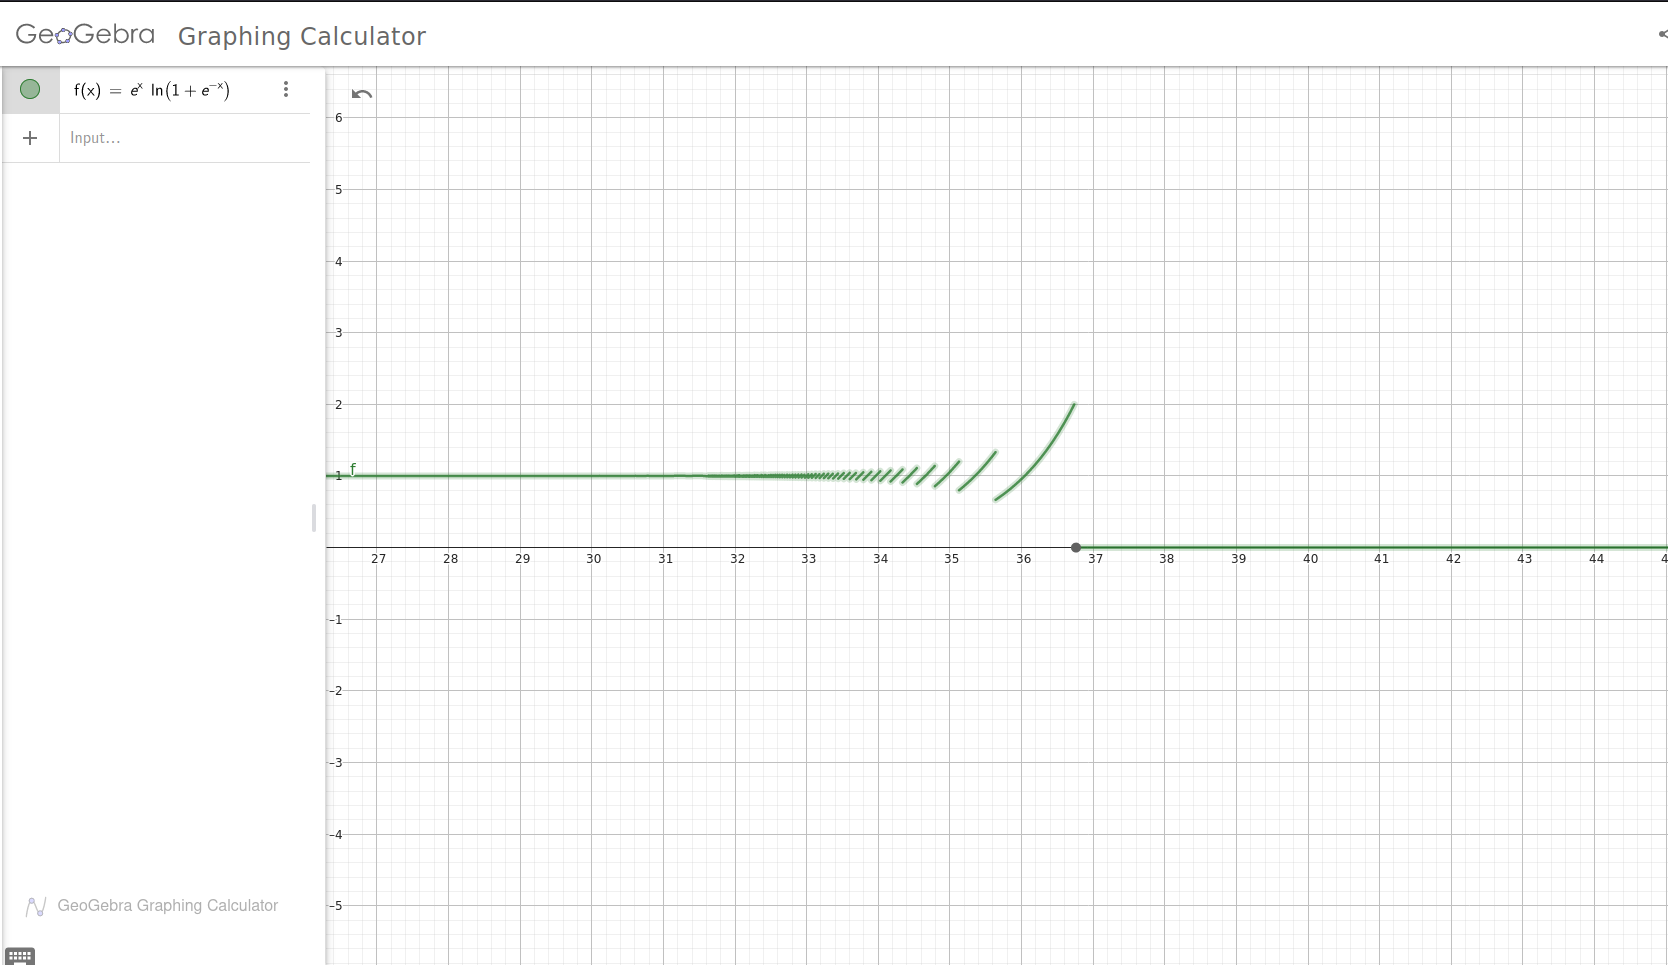
\includegraphics[width=8cm]{geo.png}
\end{figure}
\begin{figure}[htp]
  \centering
  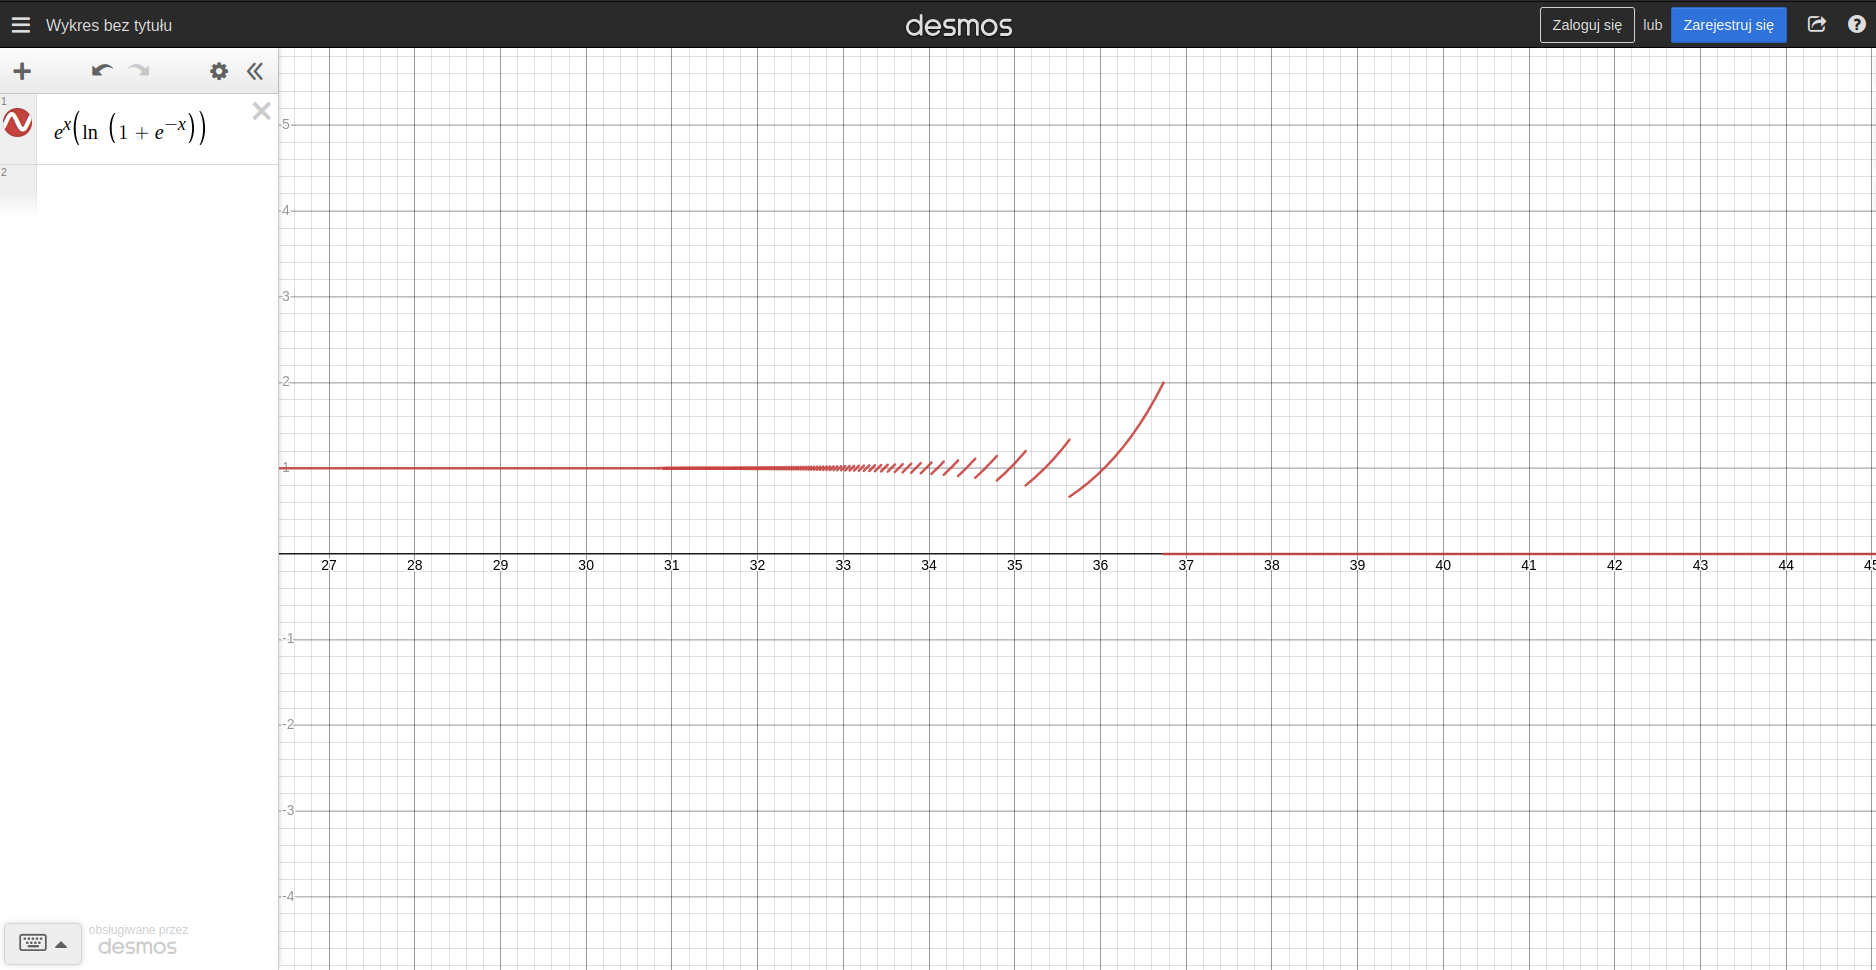
\includegraphics[width=8cm]{desm.png}
\end{figure}

\subsection{Wnioski}
\begin{enumerate}
\item Wykres nie pokrywa się z rzeczywistą granicą funkcji: \\w okolicy $x\;=\;35$ spada do 0.
\item Epsilon maszynowy dla typu Float64 jest rzędu $10^{-16}$.
\item Funkcja $g(x) = (1 + e^{-x})$ dla wartości $x > 34$ spada do epsilona maszynowego i w rezultacie spada do jedynki. Zaś $ln(1)\;=\;0$
\item Fluktuacje wykresu na odcinku $(33, 37)$ 
wynikają ze skończonej gęstości liczb blisko 1, dlatego wykres nie jest ciągły - to przeskoki funkcji $ln(g(x))$.
\item A gdy granica epsilona maszynowego pękła, wykres zwariował i po dziś dzień grasuje na lini zera.
\end{enumerate}
   

\section{Zadanie 3.}

\subsection{Opis problemu}
Rozwiązanie układu równań liniowych postaci $Ax = b$,
gdzie $A$ - macierz współczynnikow, $x$ - wektor niewiadomych, $b$ - zadany wektor wyrazów wolnych.

\subsection{Sposób rozwiązania}
W pierwszej kolejności należy przygotować dane.
\begin{enumerate}
  \item Generujemy macierze: Hilberta i Randomową
  \item Mnożymy je z wektorem $x$, aby otrzymać wektor $b$
  \item Mając zadaną macierz $A$ i wektor $b$ rozwiązujemy uklad równań dwiema metodami - eliminacji Gaussa
  oraz inwersji.
  \item Otrzymany wektor $x'$ porównujemy z oryginalnym $x$, oceniając skuteczność algorytmów.
  Żeby dało się zatabelkować liczymy normę wektora. Dla orginalnego = 1.
\end{enumerate}
\newpage

\subsection{Wyniki}
\begin{table}[h]
  \caption{Macierz Hilberta}
  \label{wyniki3}
  \centering
  \begin{tabular}{|l|l|l|l|l|}
    \hline
    \textbf{n} & \textbf{rank} & \textbf{cond} & \textbf{norm(x-inverse)} & \textbf{norm(x-gauss)}\\
    \hline
    \hline
    1 & 1 & 1.0 & 0.0 & 0.0\\ 
    \hline
    3 & 3 & 524.0567775860644 & 0.0 & 1.389554002205336e-14\\ 
    \hline
    5 & 5 & 476607.25024259434 & 7.500747052839271e-12 & 3.7629505159417226e-12\\ 
    \hline
    7 & 7 & 4.75367356583129e8 & 1.2470167790391696e-8 & 3.335463548676909e-8\\ 
    \hline
    9 & 9 & 4.931537564468762e11 & 1.3623804909529929e-5 & 1.1625490255509743e-5\\ 
    \hline
    11 & 10 & 5.222677939280335e14 & 0.025267056849832565 & 0.0005249490091577049\\ 
    \hline
    13 & 11 & 3.344143497338461e18 & 19.222187681585524 & 0.39804208446271144\\ 
    \hline
    15 & 12 & 3.674392953467974e17 & 28.44567403176546 & 18.19011830553027\\ 
    \hline
    17 & 12 & 1.263684342666052e18 & 43.36246428455144 & 56.51638468279824\\ 
    \hline
    19 & 13 & 6.471953976541591e18 & 53.325729614779235 & 42.371068229087264\\ 
    \hline
    21 & 13 & 3.290126328601399e18 & 199.22887541330184 & 258.4695319671756\\ 
    \hline
    23 & 13 & 6.313778670724671e17 & 66.2006254719103 & 59.86950653973175\\ 
    \hline
    25 & 13 & 1.3719347461445998e18 & 84.69938964854735 & 50.795974216939854\\ 
    \hline
    27 & 14 & 4.424587877361583e18 & 146.0415785777959 & 160.056977186448\\ 
    \hline
    29 & 14 & 8.05926200352767e18 & 1442.9165140119494 & 95.55951141201861\\ 
    \hline
  \end{tabular} 
\end{table}
Ta macierz jest bardzo źle uwarunkowana.
\begin{table}[h]
  \caption{Macierz Randomowa}
  \label{wyniki4}
  %\centering
  \begin{tabular}{|l|l|l|l|l|}
    \hline
    \textbf{n} & \textbf{rank} & \textbf{cond} & \textbf{norm(x-inverse)} & \textbf{norm(x-gauss)}\\
    \hline
    \hline
    5 & 5 & 1.000000000000001 & 3.8459253727671276e-16 & 0.0\\ 
    \hline
    5 & 5 & 10.000000000000004 & 5.438959822042073e-16 & 2.220446049250313e-16\\ 
    \hline
    5 & 5 & 999.9999999999565 & 3.891802844472395e-14 & 3.0787427327232494e-14\\ 
    \hline
    5 & 5 & 1.000000000610769e7 & 5.342753065833187e-10 & 5.483178137661799e-10\\ 
    \hline
    5 & 5 & 9.999080208039573e11 & 6.459691704512062e-5 & 4.939095563889871e-5\\ 
    \hline
    5 & 4 & 8.35707807125492e15 & 0.41912823576094815 & 0.40125027718625494\\ 
    \hline
    10 & 10 & 1.0000000000000013 & 8.741904837807691e-16 & 7.529898907871222e-16\\ 
    \hline
    10 & 10 & 10.000000000000014 & 7.108895957933346e-16 & 8.881784197001252e-16\\ 
    \hline
    10 & 10 & 999.9999999999897 & 1.8374778024090335e-14 & 1.9897476392944793e-14\\ 
    \hline
    10 & 10 & 1.0000000002327014e7 & 1.1867173858710762e-9 & 1.1801631451217697e-9\\ 
    \hline
    10 & 10 & 1.0000047652400917e12 & 0.00014673264147786112 & 0.00013773168775276244\\ 
    \hline
    10 & 9 & 7.555737189542885e16 & 0.610975462375536 & 0.5529051624812602\\ 
    \hline
    20 & 20 & 1.000000000000001 & 1.6910413304902302e-15 & 2.837048893407221e-15\\ 
    \hline
    20 & 20 & 9.999999999999988 & 3.1869396220701337e-15 & 3.420135685938544e-15\\ 
    \hline
    20 & 20 & 1000.0000000000271 & 1.2184483994422223e-13 & 1.154249709415512e-13\\ 
    \hline
    20 & 20 & 9.999999999786278e6 & 1.0955572491930047e-9 & 9.758161752695135e-10\\ 
    \hline
    20 & 20 & 9.999840704839703e11 & 4.9268205710210866e-5 & 2.238852829593131e-5\\ 
    \hline
    20 & 19 & 2.045522441369736e16 & 0.7176266059425617 & 0.7824065888781212\\ 
    \hline
  \end{tabular} 
\end{table}
\newpage
\subsection{Wnioski}
\begin{enumerate}
  \item Poziom uwarunkowania macierzy wpływa na dokładność wyników proporcjonalnie.
  \item W macierzy hilberta wszystkie wyniki są mocno zaburzone
  \item W macierzy zrandomizowanej dla niskiego wskaźnika cond błąd względny jest niewielki.
  \item Błąd dla macierzy zrandomizowanej nie zależy od jej rozmiaru.
\end{enumerate}

\section{Zadanie 4.}

\subsection{Opis problemu}
Wyznaczenie zer wielomianu Wilkinsona metoda "roots" z 
pakietu Polynomials.
Zbadanie poprawności wyników metodami:
\begin{enumerate}
  \item $|P(z_{k})|$
  \item $|p(z_{k})|$
  \item $|z_{k}\;-\;k|$
\end{enumerate}
Gdzie $p$ - postać iloczynowa wielomianu, $P$ - naturalna.
\\Powtórzenie esksperymentu na wielomienie, gdzie współcznynnik $-210.0$ został zmieniony na $-210.0-2^{-23}$,
\subsection{Sposób rozwiązania}
\begin{enumerate}
  \item zapisuję wielomian w postaci kanoniczej oraz iloczynowej za pomocą funkcji $Polynomial$ i $fromroots$
  \item wyznaczam miejsca zerowe wielomianu funkcją $roots$
\end{enumerate}
\newpage
\subsection{Wyniki}
\begin{table}[h]
  \caption{Sprawdzenie wyznaczonych zer na orginalnym wielomianie}
  \label{wyniki1}
  \centering
  \begin{tabular}{|l|l|l|l|}
    \hline
    \textbf{k} & \textbf{$|P(z_{k})|$} & \textbf{$|p(z_{k})|$} & $|z_{k}\;-\;k|$ \\
    \hline
    \hline
    1 & 35696.50964788257 & 5.518479490350445e6 & 3.0109248427834245e-13 \\ 
    \hline
   2 & 176252.60026668405 & 7.37869762990174e19 & 2.8318236644508943e-11 \\ 
    \hline
   3 & 279157.6968824087 & 3.3204139316875795e20 & 4.0790348876384996e-10 \\ 
    \hline
   4 & 3.0271092988991085e6 & 8.854437035384718e20 & 1.626246826091915e-8 \\ 
    \hline
   5 & 2.2917473756567076e7 & 1.8446752056545688e21 & 6.657697912970661e-7 \\ 
    \hline
   6 & 1.2902417284205095e8 & 3.320394888870117e21 & 1.0754175226779239e-5 \\ 
    \hline
   7 & 4.805112754602064e8 & 5.423593016891273e21 & 0.00010200279300764947 \\ 
    \hline
   8 & 1.6379520218961136e9 & 8.262050140110275e21 & 0.0006441703922384079 \\ 
    \hline
   9 & 4.877071372550003e9 & 1.196559421646277e22 & 0.002915294362052734 \\ 
    \hline
   10 & 1.3638638195458128e10 & 1.655260133520688e22 & 0.009586957518274986 \\ 
    \hline
   11 & 3.585631295130865e10 & 2.24783329792479e22 & 0.025022932909317674 \\ 
    \hline
   12 & 7.533332360358197e10 & 2.886944688412679e22 & 0.04671674615314281 \\ 
    \hline
   13 & 1.9605988124330817e11 & 3.807325552826988e22 & 0.07431403244734014 \\ 
    \hline
   14 & 3.5751347823104315e11 & 4.612719853150334e22 & 0.08524440819787316 \\ 
    \hline
   15 & 8.21627123645597e11 & 5.901011420218566e22 & 0.07549379969947623 \\ 
    \hline
   16 & 1.5514978880494067e12 & 7.010874106897764e22 & 0.05371328339202819 \\ 
    \hline
   17 & 3.694735918486229e12 & 8.568905825736165e22 & 0.025427146237412046 \\ 
    \hline
   18 & 7.650109016515867e12 & 1.0144799361044434e23 & 0.009078647283519814 \\ 
    \hline
   19 & 1.1435273749721195e13 & 1.1990376202371257e23 & 0.0019098182994383706 \\ 
    \hline
   20 & 2.7924106393680727e13 & 1.4019117414318134e23 & 0.00019070876336257925 \\ 
    \hline   
  \end{tabular} 
\end{table}

\begin{table}[h]
  \caption{Sprawdzenie zer na zedytowanym wielomanie}
  \label{wyniki2}
  \centering
  \begin{tabular}{|l|l|l|l|}
    \hline
    \textbf{k} & \textbf{$|P(z_{k})|$} & \textbf{$|p(z_{k})|$} & $|z_{k}\;-\;k|$ \\
    \hline
    \hline
    1 & 20259.872313418207 & 3.0131001276845885e6 & 1.6431300764452317e-13 \\ 
    \hline
   2 & 346541.4137593836 & 7.37869763029606e19 & 5.503730804434781e-11 \\ 
    \hline
   3 & 2.2580597001197007e6 & 3.320413920110016e20 & 3.3965799062229962e-9 \\ 
    \hline
   4 & 1.0542631790395478e7 & 8.854437817429642e20 & 8.972436216225788e-8 \\ 
    \hline
   5 & 3.757830916585153e7 & 1.844672697408419e21 & 1.4261120897529622e-6 \\ 
    \hline
   6 & 1.3140943325569446e8 & 3.320450195282313e21 & 2.0476673030955794e-5 \\ 
    \hline
   7 & 3.939355874647618e8 & 5.422366528916004e21 & 0.00039792957757978087 \\ 
    \hline
   8 & 1.184986961371896e9 & 8.289399860984408e21 & 0.007772029099445632 \\ 
    \hline
   9 & 2.2255221233077707e9 & 1.160747250177049e22 & 0.0841836320674414 \\ 
    \hline
   10 & 1.0677921232930157e10 & 1.7212892853670706e22 & 0.6519586830380407 \\ 
    \hline
   11 & 1.0677921232930157e10 & 1.7212892853670706e22 & 1.1109180272716561 \\ 
    \hline
   12 & 3.1401962344429485e10 & 2.8568401004080956e22 & 1.665281290598479 \\ 
    \hline
   13 & 3.1401962344429485e10 & 2.8568401004080956e22 & 2.0458202766784277 \\ 
    \hline
   14 & 2.157665405951858e11 & 4.934647147686795e22 & 2.518835871190904 \\ 
    \hline
   15 & 2.157665405951858e11 & 4.934647147686795e22 & 2.7128805312847097 \\ 
    \hline
   16 & 4.850110893921027e11 & 8.484694713563005e22 & 2.9060018735375106 \\ 
    \hline
   17 & 4.850110893921027e11 & 8.484694713563005e22 & 2.825483521349608 \\ 
    \hline
   18 & 4.557199223869993e12 & 1.3181947820607215e23 & 2.4540214463129764 \\ 
    \hline
   19 & 4.557199223869993e12 & 1.3181947820607215e23 & 2.0043294443099486 \\ 
    \hline
   20 & 8.756386551865696e12 & 1.5911084081430876e23 & 0.8469102151947894 \\ 
    \hline   
  \end{tabular} 
\end{table}
\newpage
\subsection{Wnioski}
\begin{enumerate}
  \item Metoda $roots$ nie zwróciła nam prawidłowych zer wielomianu, ponieważ podstawiając je do postaci kanonicznej
  jak i iloczynowej wielomian sie nie zeruje.
  \item Błędy mogą wynikać z reprezantacji współczynników podanego wielomiany w arytmetyce
  komputera. Arytmetyka w Float64 w języku Julia ma od 15 do 17 cyfr znaczących w
  systemie dziesiętnym, a niektóre współczynniki mają więcej cyfr.
  \item Niewielka zmiana danych rzutuje kolosalną zmianą wyników, co sugeruje, że zadanie 
  jest źle uwarunkowane. 
\end{enumerate}

\newpage

\section{Zadanie 5.}

\subsection{Opis problemu}
  Badanie rekurencyjnego algorytmu do modelowania wzrostu populacji.
  \\Sprawdzenie wyników w 3 sposobach iteracji funkcji:
  \begin{enumerate}
    \item 40 iteracji we Float32
    \item 40 iteracji we Float64
    \item 4 x 10 iteracji we Float 64, po każdych 10 obcięcie mantysy do 3 cyfr 
  \end{enumerate}
  Wzór:
  \begin{center}
    $p_{n+1} := p_{n} + r p_{n} (1 - p_{n})$
  \end{center}
\subsection{Sposób rozwiązania}
Zastosowanie wprost wzoru rekuencyjnego na opisane 3 sposoby.
\subsection{Wyniki}
  \begin{enumerate}
    \item 40 iterations Float32: 0.25860548
    \item 40 iterations Float64: 0.011611238029748606
    \item 4x10 iter. + truncate: 0.71587336
  \end{enumerate}

\subsection{Wnioski}
\begin{enumerate}
  \item Wyniki mocno zależą od precyzji arytmetyki.
  \item Niewielkie zaburzenia danych - błędy reprezentacji i zaokrągleń drastycznie wpływają na końcowy rezultat,
  ponieważ w każdej kolejnej rekursji błędy się akumulują, narastają. 
\end{enumerate}

\section{Zadanie 6.}

\subsection{Opis problemu}
Badanie iteracji równania rekurencyjnego:
\begin{center}
  $ x_{n+1} := x_n^2 + c$
\end{center}
Danych jest 7 zestawów wartości $c$ i $x_0$. Na każdym wykonujemy 40 kroków rekurencji.

\subsection{Wyniki}
1. $c = -2.0, x_0 = 1.0 : x_{40} = -1.0$\\
2. $c = -2.0, x_0 = 2.0 : x_{40} = 2.0$\\
3. $c = -2.0, x_0 = 1.99999999999999 : x_{40} = 1.2926797271549244$\\
4. $c = -1.0, x_0 = 1.0 : x_{40} = 0.0$\\
5. $c = -1.0, x_0 = -1.0 : x_{40} = 0.0$\\
6. $c = -1.0, x_0 = 0.75 : x_{40} = 0.0$\\
7. $c = -1.0, x_0 = 0.25 : x_{40} = -1.0$\\
\begin{figure}[htp]
  \centering
  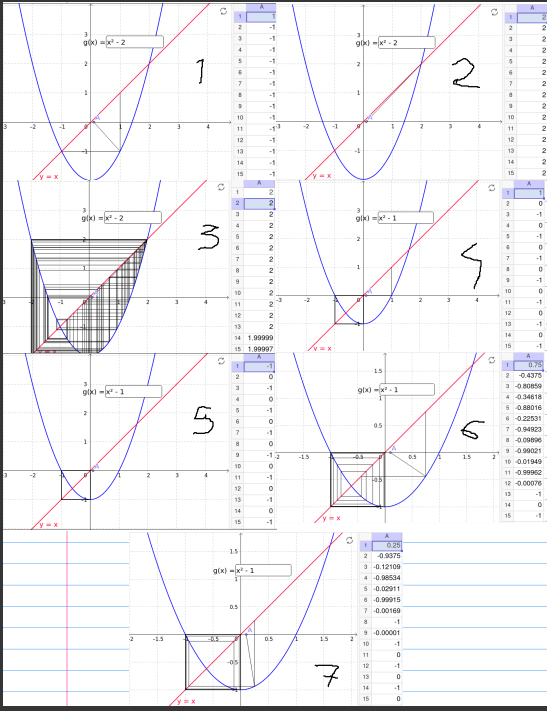
\includegraphics[width=15cm]{opus.png}
\end{figure}    
\subsection{Wnioski}
\begin{enumerate}
  \item Błędy arytmetyki mocno się akumulują. Dla wartości $x_0$ równych $0.25$ oraz $0.75$ wynik
  zbiega do liczby całkowitej dosyć szybko - po 10 iteracjach - zbiegają do liczby całkowitej.
  \item Zmiana wartości startowej z 2.0 na 1.9999999999 znacząco zaburza kolejne iteracje własnie ze wzgledu na błędy zaokrągleń.
  \item Przy takich algotymach musimy zapewnić maksymalną precyzję.
\end{enumerate}

\end{document}
